%
%     卒業論文 (2004. 1)
%                         Authorized by Jun MUKAI
%
\documentclass[12pt]{jreport}
\usepackage{b_thesis}
\usepackage{ascmac}
\usepackage{deepsection}
\usepackage{drafts}
\usepackage[dvipdfmx]{graphicx, color}
\usepackage{here}
\usepackage{tabverb}
\usepackage{tabularx}
\usepackage{array}
\usepackage{moreverb}
\usepackage{fancybox}
\usepackage{comment}
\usepackage{algorithm}
\usepackage{algorithmic}
\usepackage{indentfirst}

\pagestyle{headings}
%\pagestyle{drafts}

\topmargin=0.0truecm
\oddsidemargin=0.1truecm
\evensidemargin=0.1truecm
\textwidth=16cm
\textheight=22.5cm
\newcommand{\figurewidth}{14cm}

\title{全方位台車を用いた
\\ユーザーの位置・向き 誘導モデルの提案}

\author{小池 京太郎}                   % あなたのお名前
\teachera{今井 倫太 准教授}
\teacherb{}
\teacherc{}
\authorname{小池 京太郎}               % あなたのお名前
\date{}

\course{情報工学}
\id{60808076}                       % あなたの学籍番号

\begin{document}
\baselineskip = 20pt
\bibliographystyle{my_jalpha}
\nocite{*}
\maketitle                  %表紙がいらないときはコメントアウト

%
%     論文要旨
%
%
\jabst{
\hspace*{1zh}
\par
 本研究の目的は,人間にストレスを与えることの無い,使いやすい対話システムの実現である.単純な質問応答対話を超えた使いやすい対話システムを作るためには,対話相手に合わせて対話戦略を変えることが必要である.対話相手に合わせた対話を行うためには,人間の信念や欲求を推定することが重要である.人間の心的状態を推定する研究では,人間の散策行動から信念や欲求を推定する研究や人間の発話文から信念や欲求,意図を推定する研究がある.しかし既存研究では,
% 人間の散策行動情報と人間の発話情報の両方を用いて心的状態を推定する取り組みは少ないため,
人間の発話文による散策行動の解釈や散策行動による人間の発話の解釈を捉える方法は未だ確立されていない.本論文では,散策行動情報と人間の発話情報の両方を活用し,信念と欲求を逐次的に推定するシステムMultimodal Inference of Mind SCAIN (MIoM SCAIN)を提案する.MIoM SCAINは,散策行動情報と人間の発話情報の両方を活用して信念と欲求を推定することで,人間の発話内容による散策行動の解釈の決定や散策行動による人間の発話文の解釈を決定する.MIoM SCAINでは,独自に作成したデータセットを利用し推定システムを構築することで,人間の信念と欲求の推定を行うことができる.また,本論文では,散策行動情報と人間の発話情報の両方を活用した人間の信念と欲求の推定が有効であるかを評価する実験を行った.評価実験の結果,MIoM SCAINの推定性能が散策行動情報と人間の発話情報の一方のみから信念と欲求を推定するシステムの推定性能を上回り,散策行動情報と人間の発話情報の両方を活用した信念と欲求の推定が有効であることが示された.
}
\makejabstract
     %論文要旨
\newpage

\setcounter{page}{1}
\pagenumbering{roman}

\tableofcontents     %目次    
\listoffigures       %図目次
\listoftables        %表目次
\newpage

\setcounter{page}{1}
\pagenumbering{arabic}

\baselineskip = 20pt


%% 
%% 論文構成.ここは適宜変更する
%% 
\chapter{序論}

\par
対話システムは,発話解釈と発話生成の両方において発展を遂げており,我々の生活に浸透しつつある.しかし人間は,対話システムとの対話において不自然さやストレスを感じることも少なくない.本研究の目的は,人間に不自然さやストレスを与えることが無い,使いやすい対話システムの実現である.

\par
対話システムと人間との対話では,対話システムが対話相手の心的状態を推定し,それを考慮した対話を行うことが重要である.
人間は,気分が落ち込んでいる対話相手の発話に対してネガティブな発話解釈をしたり,励ましの言葉をかけるように,対話相手の心的状態によって相手の発話の解釈を変えたり,自身の発話の内容を変えている.また,相手が知らないことについて詳しく説明したり,相手が好むことについて話を掘り下げる.対話システムにおいても,人間と同様に対話相手の心的状態に合わせて,発話解釈を変えたり,自身の発話の内容を変えることで,より自然でありストレスの少ない対話を実現することができる.つまり,対話相手に合わせた臨機応変な発話解釈や発話生成により対話における不自然さやストレスをなくすためには,対話相手の心的状態を推定することが必要となる.


\par
人間の心的状態を推定する研究には,人間の散策行動情報から心的状態を推定する研究や発話情報から心的状態を推定する研究が存在する.人間の散策行動情報から心的状態を推定する研究は,代表的には,環境の状態と環境中を移動する人間の散策行動や観測状況をベイズ推定\cite{alma9926464316904034}に適用し,環境中を移動する人間の信念と欲求を推定する研究 \cite{baker2011bayesian}があげられる.信念はどのようなことを考えているかということを意味し,欲求は何を望んでいるかということを意味する.発話情報から心的状態を推定する研究では,代表的には,人間の発話情報から得られた事象を信念と捉え,考えられる欲求の候補を生成し,尤もらしい欲求を基に発話者の意図を推定する研究 \cite{高橋拓誠2015bdi}があげられる.また,ユーザの信念,欲求および意図を考慮することによる検索精度の向上のために検索クエリへの入力から人間の信念,欲求および意図を推定する研究 \cite{10.1007/978-3-642-02481-8_4}や,機械翻訳において,ユーザの信念によって翻訳の粒度や表現を変えるために,入力文からユーザの信念を推定する研究\cite{farwell1997user}も存在する.

% 教師の発話から学習者の心的状態を推定する

\par
従来研究では,散策行動情報のみから人間の信念と欲求を推定する研究や人間の発話情報のみから人間の信念と欲求を推定する研究は存在した.しかし,散策行動情報と人間の発話情報の両方を活用し人間の信念と欲求を推定する取り組みは少ない.従来研究における信念と欲求の推定は,遠くから散策行動を観測している場合や立ち止まって対話をしている場合というように,散策行動情報のみが観測される場合や人間の発話情報のみが観測される場合には有効である.しかし実世界では,散策行動情報と人間の発話情報の両方が観測されることが多く,人間の発話情報によって散策行動情報の解釈が依存して決まったり,散策行動情報によって人間の発話情報の解釈が依存して決まることがある.
\begin{figure}[htbp]
  \begin{center}
    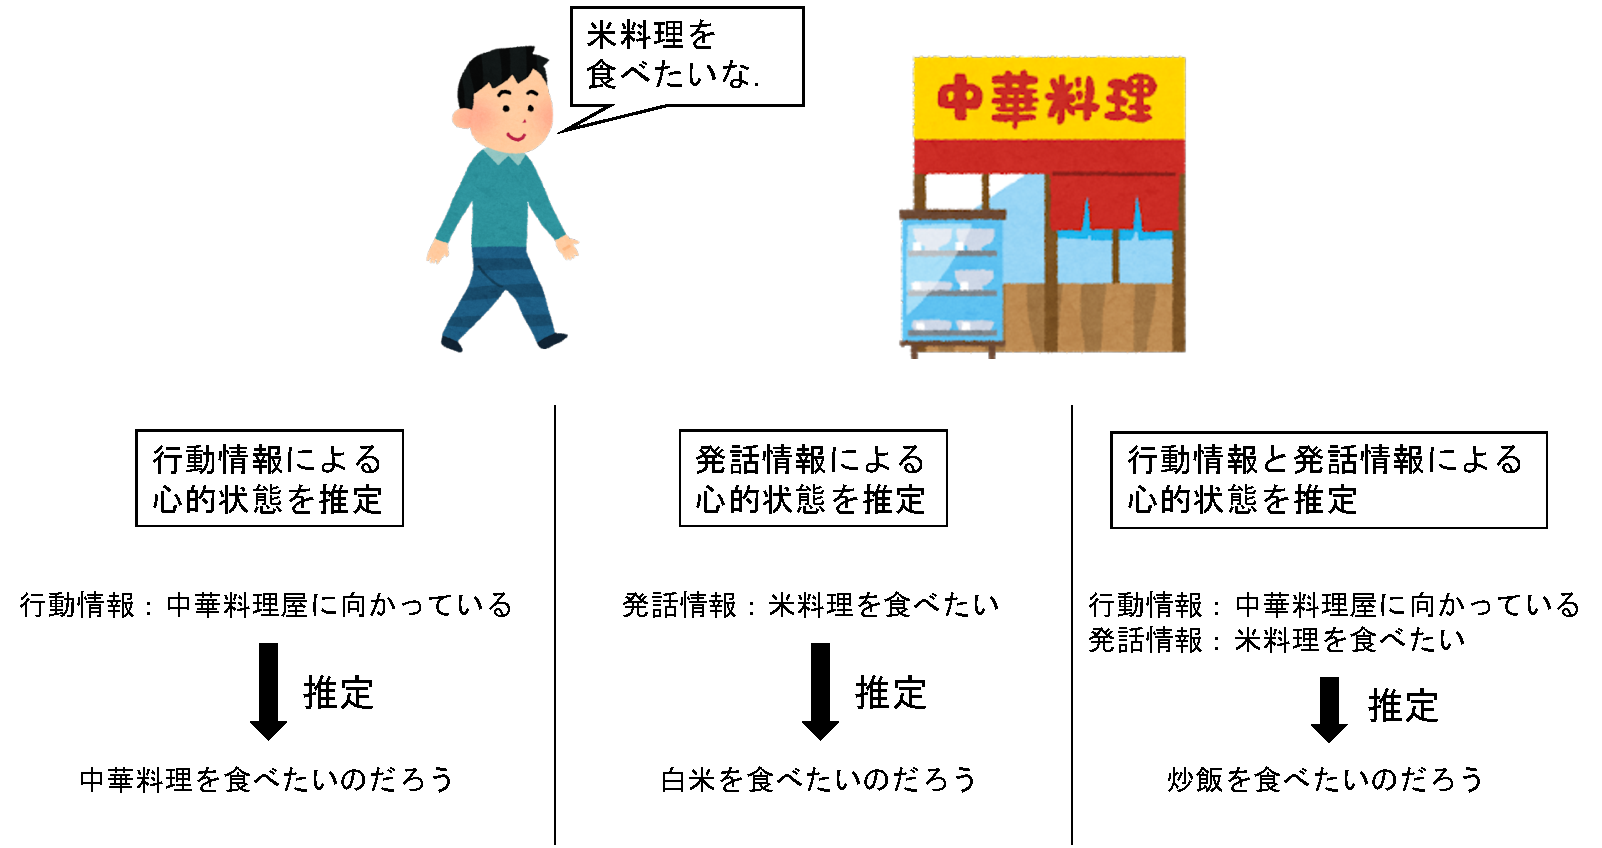
\includegraphics[scale=0.5]{./figure1.pdf}
    \caption{散策行動情報と人間の発話情報の相互作用を考慮した信念と欲求の推定}
    \label{fig:fig1}
  \end{center}
\end{figure}
例えば,図\ref{fig:fig1}の左側の状況において,散策行動情報は「料亭と中華料理屋が並ぶ飲食店街に向かっている」と解釈できるが,図\ref{fig:fig1}の右側の状況のように「魚料理を食べたいな」という人間の発話情報が観測された時,散策行動情報は「料亭に向かっている」と解釈される.
従来研究では,散策行動情報と人間の発話情報の両方が観測される場合においては,人間の発話情報による散策行動情報の解釈の決定や,散策行動情報による人間の発話情報の解釈の決定をすることが難しい.つまり,散策行動と人間の発話の両方が観測される場合における従来研究における信念と欲求の推定では,散策行動と人間の発話の相互依存の考慮による推定性能の向上の可能性が低いことが予想される.
% 従来研究では,行動情報のみから人間の心的状態を推定する研究や発話情報のみから人間の心的状態を推定する研究は存在した.しかし,行動情報と発話情報の両方を活用し人間の心的状態を推定する研究はない.従来研究における心的状態の推定は,遠くから行動を観測している場合や立ち止まって対話をしている場合というように,行動情報のみが観測される場合や発話情報のみが観測される場合には有効である.しかし実世界では,図\ref{fig:fig1}にように行動情報と発話情報の両方が観測されることが多く,発話情報によって行動情報の解釈が変わったり,行動情報によって発話情報の解釈が変わることがある.
% \begin{figure}[htbp]
%   \begin{center}
%     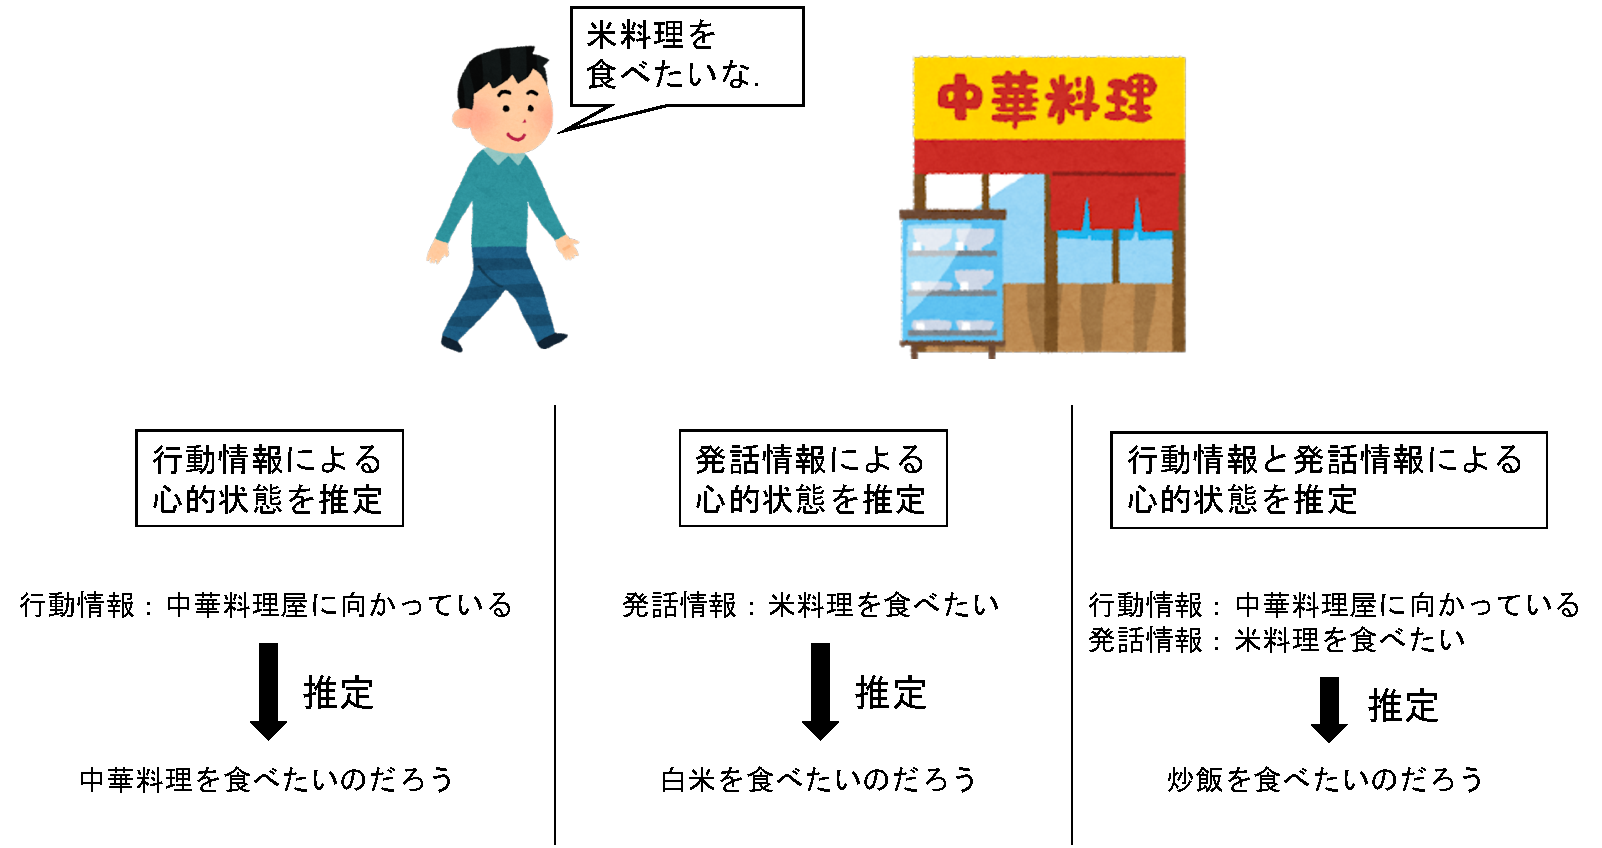
\includegraphics[scale=0.58]{./figure1.pdf}
%     \caption{心的状態の推定.人間が食事をとるために飲食店に向かう場面において,3通りの条件で心的状態を推定する.図の左側は,行動情報のみを活用して心的状態を推定した場合,図の中央は発話情報のみを活用して心的状態を推定した場合,図の右側は行動情報と発話情報の両方を活用して心的状態を推定した場合を表す.}
%     \label{fig:fig1}
%   \end{center}
% \end{figure}
% また行動情報のみを活用して「中華料理を食べたいのだろう」という心的状態を推定したり発話情報のみを活用して「白米を食べたいのだろう」という心的状態を推定するのに対し,行動情報と発話情報の両方を活用して「炒飯を食べたいのだろう」という心的状態を推定するように,行動情報と発話情報の両方を活用することにより,発話情報による行動情報の解釈の変化や行動情報による発話情報の解釈の変化を捉えることが可能となり,より多くの情報を基に推定を行うことができる.
% 従来研究では,行動情報と発話情報の両方が観測される場合においては,発話情報による行動情報の解釈の変化や,行動情報による発話情報の解釈の変化を捉えることが難しい.つまり,行動と発話の両方が観測される場合における従来研究における心的状態の推定では,行動と発話の相互作用の考慮による推定性能の向上の可能性が低いことが予想される.

\par
本研究では,散策行動情報と人間の発話情報の両方から人間の心的状態の一部である信念および欲求を逐次的に推定するシステムMultimodal Inference of Mind SCAIN (MIoM SCAIN)を提案する.MIoM SCAINは,人間の信念および欲求の推定において,信念と欲求の組み合わせをを一つに断定するのではなく,同時に複数保持し,やり取りの中で動的に推定する.MIoM SCAINは,散策行動情報と人間の発話情報の両方を推定に活用し,ベイズ推定によって人間の信念および欲求を逐次的に推定する.散策行動情報と人間の発話情報の両方を推定に活用することにより,図\ref{fig:fig1}の右側の状況における推定のように,人間の発話情報による散策行動情報の解釈の決定や散策行動情報による人間の発話情報の解釈を決定を行い,散策行動情報と人間の発話情報の相互依存を考慮した推定が可能となる.実験では,独自で作成したデータセットを利用し,MIoM SCAINにより信念と欲求の推定を行い,散策行動情報と人間の発話情報の両方を推定に活用することが有効であるかを評価する.

\par
本論文の構成は以下の通りである.第二章では,関連研究においてどのように人間の信念や欲求を推定していたかを述べる.第三章では,人間の散策行動情報と人間の発話情報から信念と欲求を推定するシステムMIoM SCAINを提案する.第四章では,MIoM SCAINと散策行動情報もしくは人間の発話情報のみから信念と欲求を推定するシステムを用いて実験的に評価し,第五章では評価結果について考察する.第六章では,MIoM SCAINにおける今後の課題について述べる.最後に,第七章で本論文を締めくくる.

\chapter{背景}
本章では問題設定および作成すべきモデルについて記述する.

\section{問題設定}

\subsection{全方位台車について}
全方位台車とは,ホイールを等角度間隔で3個以上配置した移動機構を持つ車両のことである.
全方位台車は並進移動や回転により小さなスペースても素早く移動できるので,
今後一般家庭や公共施設にも搬送なとの用途で普及すると思われる.
例えば今井らは病院内ロボット搬送システムの開発を研究しているが,
ここで用いられているロボットには全方位移動機構が採用されている\cite{Imai}.
\par
全方位台車の普及を受けて,動作に関する研究が多く行われている.
例えば,L.Huangらは90度間隔でホイールを4輪持つ全方位台車を設計した.
また動作アルゴリズムを作成し,直線や円の軌跡をトレースして動けるか動作検証が行われた\cite{L}.
多田隈らは全方位台車を任意の方向へ任意の回転速度で移動させるための,ホイールの回転速度
決定に関する研究が行われた\cite{Tada}.
本稿の全方位台車の動作はその回転速度決定の行列式を元に設計されている.
\par
全方位台車の位置座標取得は大きく分けて,全方位台車に搭載されたデバイスにより行う物と外部のシステムから取得するものがある.
全方位台車に搭載するものとしては,レーザーレンジファインダによるSLAMといったものがある.
外部のシステムでは,モーションキャプチャが一般的であると思われる.

\subsection{全方位台車による人の位置向き誘導の必要性}
\label{yuudou}
人間のタスクを全方位台車がサポートするに当って,全方位台車により人間に場所や方向を指示する必要がある場面が考えられる.
例えば荷物を置き場まで運ぶタスクにおいては,人間に運ぶべき荷物やそれを置く場所・方向を指示することが求められる.
このようなタスクにおいて人間をサポートする場合,全方位台車により人の位置・向きの誘導が行える必要がある.

\section{作成すべきモデル}
\ref{yuudou}において説明した全方位台車による人の位置・向き誘導を行うためには,
全方位台車の位置・向きに対して人がどのような位置・向きに誘導されるかを示す
モデルが必要となる.
本稿ではそのモデルを全方位台車による人の位置・向き誘導の実験を通して作成する.
また,作成したモデルに従い全方位台車の動作に対して予測される人の動作を
図示するツールを作る.
これにより全方位台車の誘導の動作を改良することが出来る.
\chapter{提案}
\par
本論文では,行動情報と発話情報の両方を活用する心的状態推定システムMultimodal Inference of Mind(MIoM)を提案する.MIoMは,人間の信念や行動,発話および人間が存在する環境の状態を基に心的状態を推定する.行動情報と発話情報の両方を心的状態の推定に活用することで,発話による行動の解釈の変化や行動による発話に解釈の変化を捉え,行動情報と発話情報の相互作用を考慮して心的状態を推定する.

\par
MIoMは,環境の状態や人間の心的状態を部分的に観測可能なマルコフ決定過程(POMDP)として表される.また,心的状態とその尤度を持つパーティクルフィルタとして表され,心的状態を一意に決め付けるのではなく同時に複数保持し,時刻が経過する度に各パーティクルの尤度を更新していく.各時刻おける人間の信念や行動,発話および人間が存在する環境の状態をベイズの定理に適用し,人間が観測できていない環境領域についての信念と欲求を逐次的に推定する.


\section{関連研究との相違点}
\par
MIoMと関連研究との相違点は,行動情報と発話情報の両方を活用したマルチモーダルな心的状態推定を行う点である.MIoMは,行動情報と発話情報の両方を活用して心的状態を推定することで,発話による行動の解釈の変化や行動による発話の解釈の変化を捉え,行動情報と発話情報の相互作用を考慮した推定が可能となる.MIoMは,関連研究における問題点を解消するシステムとなっている.


\section{アルゴリズム}

\par
MIoMにおける推定処理の流れをを図\ref{fig:sys_arc}に示す.
\begin{figure}[htbp]
  \begin{center}
    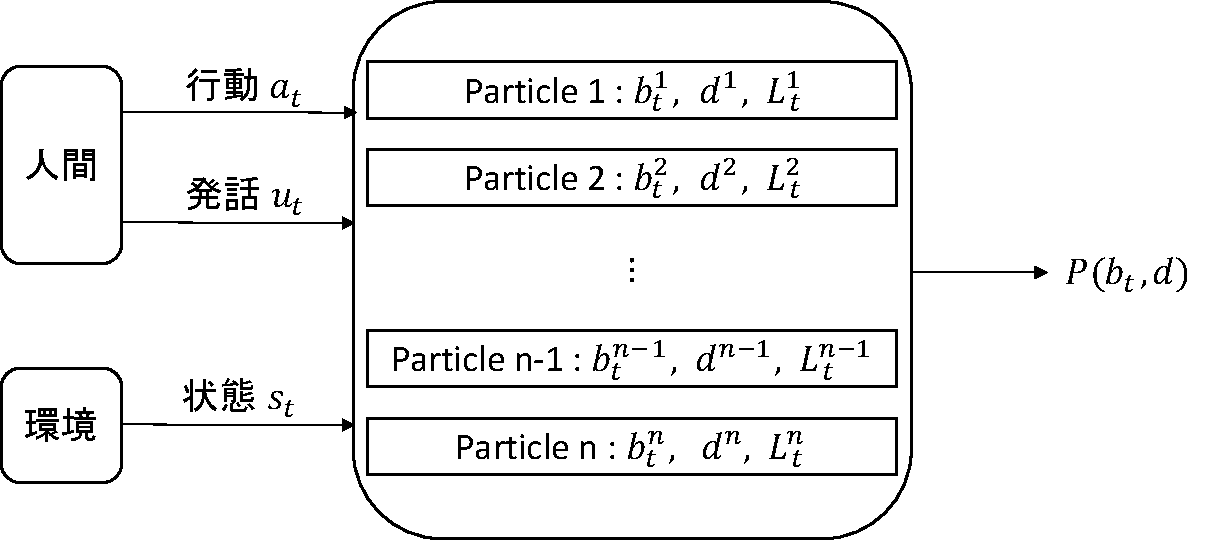
\includegraphics[scale=0.75]{./bt1.pdf}
    \caption{MIoMによる推定処理}
    \label{fig:sys_arc}
  \end{center}
\end{figure}
図\ref{fig:sys_arc}に示すように,MIoMは時刻$t$における人間の行動$a_t$,発話$u_t$および環境の状態$s_t$から信念と欲求の確率を出力する.MIoMは信念$b_t$と欲求$d$の組み合わせとその尤度$L$を持つパーティクルフィルタとして表現され,$a_t,u_t,s_t$を基にそれぞれのパーティクルの尤度$L^k$が更新される.ここで,尤度$L^k$は次のように表すことができる.
\begin{equation}
  \begin{split}
  \label{pf}
  L^k=P(b_t^k,d^k|s_{1:t},a_{1:t-1},u_{1:t-1})
  \end{split}
\end{equation}
ここで,$u_{1:t-1}$は,時刻$1$から時刻$t-1$までの人間の発話履歴,$P(b_t,d|s_{1:t},a_{1:t-1},u_{1:t-1})$は,$s_{1:t},a_{1:t-1}およびu_{1:t-1}$から計算される$b_t$と$d$の確率である.

\par
図\ref{fig:miom}にMIoMにおけるベイズ推論の様子を示す.
\begin{figure}[htbp]
  \begin{center}
    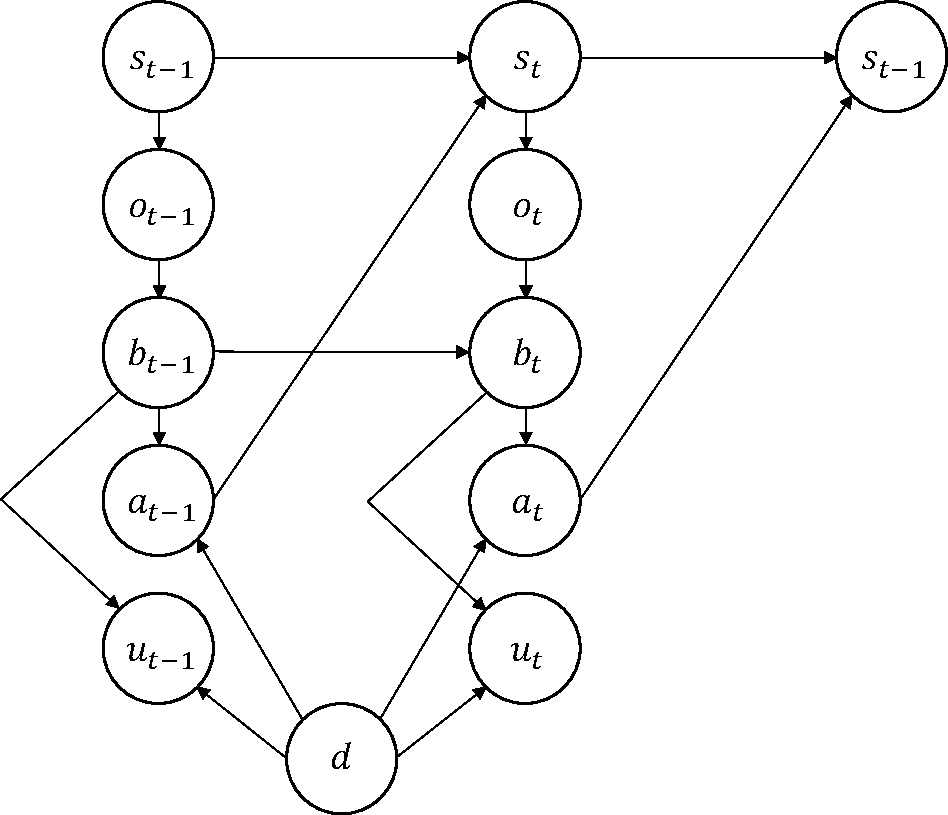
\includegraphics[scale=0.85]{./miom.pdf}
    \caption{MIoMにおけるベイズ推定}
    \label{fig:miom}
  \end{center}
\end{figure}
MIoMにおけるベイズ推論では,BToMと同様に時刻$t$における環境の状態$s_{t}$を基に人間の観測状況$o_{t}$が決まる.また,$o_{t}$を基に人間の信念$b_{t}$が決まり,$b_{t}$と人間の欲求$d$から人間の行動$a_{t}$が決まる.それに加え,MIoMでは$b_t$と$d$から人間の発話$u_t$が決まる.また$a_{t}$起こることにより,環境の状態は$s_{t+1}$に変化し,人間の観測状況,信念,行動および発話が再起的に決定される.MIoMでは各パーティクルの尤度である式(\ref{pf})を計算することを目的としている.以下に,式(\ref{pf})にベイズの定理を適用した過程を示す.

\begin{equation}
  \begin{split}
  \label{eq_miom}
  L^k&=P(b_t^k,d^k|s_{1:t},a_{1:t-1},u_{1:t-1})\\
  &\propto P(b_t^k,d^k,s_{1:t},a_{1:t-1},u_{1:t-1})\\
  &= \sum_{b_{t-1}^k,o_t}P(b_t^k,d^k,s_{1:t},a_{1:t-1},u_{1:t-1},b_{t-1}^k,o_t)\\
  &= \sum_{b_{t-1}^k,o_t}P(b_t^k|d^k,s_{1:t},a_{1:t-1},u_{1:t-1},b_{t-1}^k,o_t)\cdot P(d^k,s_{1:t},a_{1:t-1},u_{1:t-1},b_{t-1}^k,o_t)\\
  &= \sum_{b_{t-1}^k,o_t}P(b_t^k|b_{t-1}^k,o_t)\cdot P(o_t|d^k,s_{1:t},a_{1:t-1},u_{1:t-1},b_{t-1}^k)\\
  &\hspace{5cm} \cdot P(d^k,s_{1:t},a_{1:t-1},u_{1:t-1},b_{t-1}^k)\\
  &= \sum_{b_{t-1}^k,o_t}P(b_t^k|b_{t-1}^k,o_t)\cdot P(o_t|s_t)\cdot P(s_t|s_{t-1},a_{t-1})\\
  &\hspace{3cm} \cdot P(a_{t-1}|b_{t-1}^k,d^k)\cdot P(u_{t-1}|b_{t-1}^k,d^k)\cdot P(b_{t-1}^k,d^k,s_{t-1},a_{t-2},u_{t-2})\\
  \end{split}
\end{equation}


ここで,$P(b_t^k|b_{t-1}^k,o_t)$は人間の観測$o_t$によって$k$番目のパーティクルの信念$b_t^k$が更新される確率,$P(o_t|s_t)$は環境の状態$s_t$において人間が観測状況$o_t$を得る確率,$P(s_t|s_{t-1},a_{t-1})$は環境の状態$s_{t-1}$において人間が行動$a_{t-1}$を起こした時に環境の状態が$s_{t}$になる確率,$P(a_{t-1}|b_{t-1}^k,d^k)$は$k$番目のパーティクルが信念$b_{t-1}^k$,欲求$d^k$を持っている時に行動$a_{t-1}$を起こす確率,$P(u_{t-1}|b_{t-1}^k,d^k)$は$k$番目のパーティクルが信念$b_{t-1}^k$,欲求$d^k$を持っている時に発話$u_t$を起こす確率,$P(b_{t-1}^k,d^k,s_{t-1},a_{t-2},u_{t-2})$は時刻$t-1$における$k$番目のパーティクルの尤度である.式(\ref{eq_miom})より,$L^k$は再起関数として表すことができ,初期値$P(b_1,d,s_1,a_0,u_0)$を決めることで更新することができる.また,$P(b_t^k|b_{t-1}^k,o_t)$,$P(o_t|s_t)$,$P(s_t|s_{t-1},a_{t-1})$,$P(a_{t-1}|b_{t-1}^k,d^k)$および$(u_{t-1}|b_{t-1}^k,d^k)$の乗算として表すことができる.

\par
% それぞれの生起確率がどのように計算されるかを記載
MIoMでは,各時刻における$P(b_t^k|b_{t-1}^k,o_t)$,$P(o_t|s_t)$,$P(s_t|s_{t-1},a_{t-1})$,$P(a_{t-1}|b_{t-1}^k,d^k)$および$(u_{t-1}|b_{t-1}^k,d^k)$を計算し,乗算することで,その時刻における信念と欲求の尤度を計算する.$P(b_t^k|b_{t-1}^k,o_t)$は既に人間が$b_t^k$を観測しているかどうかを$o_t$によって計算する.
$P(a_{t-1}|b_{t-1}^k,d^k)$は信念$b_{t-1}^k$と欲求$d^k$を基に上,下,左,右の4方向の確率を計算する.$(u_{t-1}|b_{t-1}^k,d^k)$はWord2Vecにより発話$u_t$を分散表現に変換した後,信念$b_{t-1}^k$と欲求$d^k$との類似度を基に計算する.

% \chapter{?V?X?e?????v}

?{???????????p????V?X?e????,?U???f?[?^?擾?V?X?e??,?????p?V?X?e??,????V?X?e??,
?U??????m?F?V?X?e????4??????.
?U???f?[?^?擾?V?X?e?????l????m???U?????????f?[?^??
???[?V?????L???v?`??????擾??,???O?f?[?^???????????.
?????p??V?X?e?????S?????????[?V?????L???v?`????A???????V?X?e??????
???g???u???W??p?x??擾??,?????]????????.
???????????O?f?[?^??L?^????o????s??.
????p??V?X?e???????O?f?[?^????o??,?S???????U???????l???
??u??p?x??`????.
?U??????m?F?V?X?e???????O?f?[?^????o??,????f?[?^??p????U????s????????
?U???????l????????f??????\????,?????`????.
?{?????L??V?X?e?????v???????????.

\section{?U???f?[?^?擾?V?X?e??}
?U???f?[?^?擾?V?X?e????\???}??}\ref{getsystem}????.
???[?V?????L???v?`?????W???[??,???O?f?[?^??????W???[?????莞????????s????.
???[?V?????L???v?`?????W???[?????Z???T?[???u???W??????????J????????擾????.
???O?f?[?^??????W???[?????U????????s???l????u???????f?[?^??O?t?@?C??????????.

\begin{comment}
\begin{figure}[!h]
\begin{center}

\includegraphics[width=8cm,height=8cm]{getsystem.eps}
\caption{?U???f?[?^?擾?V?X?e??}
\label{getsystem}
\end{center}
\end{figure}
\end{comment}

\subsection{???[?V?????L???v?`?????W???[??}
?uNatural Point Tracking tools?v????C?u??????p???邱?????,
?Z???T?[???u,?p?x??????????p???邱????o????.
??????W???[?????????p????l????????2???????W??擾??,
?????????u???????Z?o??s??.

\subsection{???O?f?[?^??????W???[??}
???[?V?????L???v?`?????W???[?????????擾?????f?[?^??e?L?X?g?t?@?C??????????.
???O????????????у^?C???X?^???v??t??,???o?????????????????o????
?e??????????????.


\section{?????p?V?X?e??}
?????p?V?X?e????\???}??}\ref{expsystem}?????.
??????????????W???[??????s??????,
???[?V?????L???v?`?????W???[??,???O?f?[?^??????W???[??,?S???????????W???[????
3?????W???[?????莞????????s????.
??????????W???[?????U???f?[?^?擾?????????^??????????????????.
???[?V?????L???v?`?????W???[????O?????l?????.
???O?f?[?^??????W???[?????????????L?^?????????,???????l???U???????f?[?^????o?????s??.
?S???????????W???[?????,???O?f?[?^??????W???[??????o??????W???W?_????ъp?x??
?????S?????????????????K?v????[?^?[???]?l????Z??s??.
???,???Z?????S????????????M??p??????M????.

\begin{comment}
\begin{figure}[!h]
\begin{center}

\includegraphics[width=8cm,height=8cm]{expsystem.eps}
\caption{?????p?V?X?e??}
\label{expsystem}
\end{center}
\end{figure}
\end{comment}


\subsection{??????????W???[??}
?????????????????????????????,?^?C?~???O?????^??????????????????.
?^?C?~???O??????????O?t?@?C????^?C???X?^???v?????????p????.

\subsection{???O?f?[?^??????W???[??}
???[?V?????L???v?`??????擾?????f?[?^??e?L?X?g?t?@?C???????????????,
?U???f?[?^????O????o????s??.
???O????o??????^?C???X?^???v?????????p????,???O???????????
??????I???v???????????????????.

\subsection{?S??????????W???[??}
?S???????4???z?C?[?????????????]????w??UDP????M??,?C???_??C???p?x??S???????????????.
?z?C?[?????]???v?Z????????????L?q????.





\section{????V?X?e??}
????V?X?e????\???}??}\ref{anasystem}?????.
???O?f?[?^??????W???[??,?`???W???[?????莞????????s????.
???O?f?[?^??????W???[?????S??????,????????f?[?^????o??.
?`???W???[???????O?f?[?^??????o?????S???????????????u???????2?????}?b?v??`????.
????\????W??????????????U????????W???????u??????`????.
???????S???????????????????????_???@???邱????o??,
????O???`????\????.

\begin{comment}
\begin{figure}[!h]
\begin{center}

\includegraphics[width=8cm,height=8cm]{anasystem.eps}
\caption{????V?X?e??}
\label{anasystem}
\end{center}
\end{figure}
\end{comment}

\subsection{???O?f?[?^??????W???[??}
?????V?X?e????U???f?[?^?擾?V?X?e???????????S??????????????
??u?E?p?x??f?[?^??e?L?X?g?t?@?C????????o??.
???O????o??????^?C???X?^???v?????????p????,???O???????????
??????I???v?????????`?悳????????????.


\subsection{?`???W???[??}
OpenGL??p???邱?????,?S???????????????u???????2?????}?b?v??`????.
?U????????W???????u??,??????????W???????????????`????.



\section{?U??????m?F?V?X?e??}
?U??????m?F?V?X?e????\???}??}\ref{toolsystem}?????.
?U???\?????W???[??,?`???W???[??,???O?f?[?^??????W???[?????莞????????s????.
???O?f?[?^??????W???[??????????u?E????????o??.
?U???\?????W???[?????,???O??????o?????S???????U????????????l?????????
?U?????????f????????????u???W??p?x??v?Z????.
?`???W???[?????S???????????????????l???????`????.

\begin{comment}
\begin{figure}[!h]
\begin{center}

\includegraphics[width=8cm,height=8cm]{toolsystem.eps}
\caption{?U??????m?F?V?X?e??}
\label{toolsystem}
\end{center}
\end{figure}
\end{comment}

\subsection{?U???\?????W???[??}
?S????????u?E??????????\???????l?????ΓI???u?E??????Z?o????.
?????,??????????????????f????p????.


\subsection{???O?f?[?^??????W???[??}
????V?X?e??????l?????.


\subsection{?`???W???[??}
OpenGL??p???邱?????,?S??????????U???\?????W???[????Z?o????
?l????u?E?????E?????2?????}?b?v??`????.
?U????????W???????u??,??????????W???????????????`????.


%%\chapter{実装}


\chapter{システムの実装}
本章では,本研究において用いる誘導データ取得システム,実験用システム,分析システム,
誘導動作確認システムの実装について説明する.
また,本研究で用いたハードの仕様やハードに関する実装も併せて説明する.

\section{使用したハードの仕様}
\subsection{全方位台車}
\par
本稿では全方位台車として三菱電機特機システム株式会社の小型全方位ロボット(図\ref{mitubisiomni})を用いた.
スペックは表\ref{mitubisispec}のようになっている.

\begin{comment}
\begin{figure}[!h]
\begin{center}

\includegraphics[width=5cm,height=5cm]{mitubisiomni.eps}
\caption{小型全方位ロボット}
\label{mitubisiomni}
\end{center}
\end{figure}
\end{comment}

\begin{table}[!h]



\begin{center}
\begin{tabular}{|c|c|}


\hline
型名 & MDT-RO-02\\
\hline
外形寸法 & 直径390mm,高さ151mm \\
\hline
重量 & 約8kg(バッテリー含む) \\
\hline
電源 & 模型用DC7.2V ニッケル水素バッテリー\\
\hline
標準モーター & マブチモータ RS-380シリーズ \\
\hline
ギア比 & 1/36(6.5r/s:出力軸)\\
\hline
最高移動速度(無負荷/平地走行時)  & 約1.5km/h\\
\hline
積載重量 & 15kg以下(設置面の状態による)\\
\hline
通信方式 & 無線LAN(2.4GHz)\\
\hline
\end{tabular}
\end{center}

\caption{全方位台車のスペック}
\label{mitubisispec}
\end{table}


この全方位台車は周囲に90°ごとに4個のホイールが配置されており,また無線受信機を搭載している.
その受信機とUDP通信を行い,4個のホイールそれぞれの回転数を指定することにより動作する.


\subsection{モーションキャプチャシステム}
本稿では,全方位台車や人の位置を取得するシステムとして
OptiTrack社のモーションキャプチャシステムを用いた.
ソフトウェアはNatural Point Tracking Tools,ハードウェアはモーションキャプチャカメラ「S250e」を用いた.
S250eの写真を図\ref{S250e}に示す.
また,S250eのスペックを表\ref{S250espec}に示す.

\begin{comment}
\begin{figure}[!h]
\begin{center}

\includegraphics[width=5cm,height=5cm]{S250e.eps}
\caption{モーションキャプチャカメラ「S250e」}
\label{S250e}
\end{center}
\end{figure}
\end{comment}


\begin{table}

\begin{center}
\begin{tabular}{|c|c|c|c|}


\hline
幅 & 8.1cm & 遅延時間 & 4ms \\
\hline
高さ & 8.0cm & 精度 & 1mm以下 \\
\hline
奥行 & 6.8cm & レンズ視野角 & 43°,56° \\
\hline
重さ & 431g & シャッタータイプ & グローバル\\
\hline
フレームレート & 250-30(調整可能) & IRリング & 96個のLED付 \\
\hline
MJPEGフレームレート & 125-30(調整可能) & インターフェース & Ethernet/PoE \\
\hline
解像度 & 832×832 & マウント & 1/4"-20 \\
\hline
\end{tabular}
\end{center}

\caption{S250eのスペック}
\label{S250espec}
\end{table}

このモーションキャプチャシステムでは,赤外線を反射するセンサを図\ref{sensorplate}のように3個一組の状態にした剛体プレートの位置及び向きの情報が得られる.
3個一組の状態をあらかじめ登録しておき,それらの相対的位置により各々のセンサプレートの個体認識をしている.

\begin{comment}
\begin{figure}[!h]
\begin{center}

\includegraphics[width=5cm,height=5cm]{sensorplate.eps}
\caption{センサプレート}
\label{sensorplate}
\end{center}
\end{figure}
\end{comment}


\section{ハードの利用}
本研究ではハードとしてモーションキャプチャおよび全方位台車を用いている.
ここではそれらの実装について記述する.
\subsection{モーションキャプチャ}
本研究ではモーションキャプチャシステムとしてOptiTrack社の
Natural Point Tracking Toolsというソフトウェアを用いている.
このソフトウェアでは以下の関数を用いてセンサのデータを取得する.
\\
\\
\verb|TT_TrackableLocation(TRUCK,&x,&y,&z,&qx,&qy,&qz,&qw,&yaw,&pitch,&roll);|
\\
\\

\begin{itemize}
\item TRUCK
\begin{itemize}
\item 予め定義したセンサプレートの番号(int値)
\item どのセンサプレートの位置情報を取得するか指定
\end{itemize}

\item \verb|&x,&y,&z|
\begin{itemize}
\item センサの位置情報を格納する変数をここで指定
\end{itemize}

\item \verb|&qx,&qy,&qz|
\begin{itemize}
\item 回転演算がしやすい虚数を用いた位置情報
\item 本研究では用いない
\end{itemize}

\item \verb|&yaw,&pitch,&roll|
\begin{itemize}
\item センサプレートの向き
\item 本研究ではyawのみを用いる
\end{itemize}
\end{itemize}

\subsection{全方位台車}
\subsubsection{モーター値の送信}
本研究で用いた全方位台車はUDP通信により-100~100のモーター値を送信しホイールを回転させることで動作する.
具体的には"RXT000GM,モーター値,モーター値;"という文字列を送信する.
ホイールが2個1組となっており,上記の文字列を2つのソケットにそれぞれ送信することにより
合計4個のホイールを動作させる.
数字を文字列に組み込むのには,sprintf関数を用いた.

\subsubsection{モーター値の計算}
図\ref{omniact}「絶対座標系における全方向移動車の制御」
の行列式を基に,モーター値の計算プログラムを実装した\cite[p15]{Tada}.

\begin{comment}
\begin{figure}[!h]
\begin{center}
\includegraphics[width=13cm,height=8cm]{omniact.eps}
\caption{絶対座標系における全方位台車の制御}
\label{omniact}
\end{center}
\end{figure}
\end{comment}

\newpage

モーター値を求める際には角度を補正する計算と距離を補正する計算をそれぞれ行った.
角度を補正するプログラムの擬似コードを以下に示す.

\vspace{4zh} 
\hrule width 15cm
\begin{verbatimtab}	
IF モーターの角度差が正方向へ180°以内 OR 負方向へ180°より大きい THEN
		IF モーターの角度差が負方向へ180°より大きい THEN
			角度差=360-角度差の絶対値
	
		各ホイールのモーター値 = |角度差*定数|
		
IF モーターの角度差が負方向へ180°以内または正方向へ180°より大きい THEN
		IF モーターの角度差が正方向へ180°より大きい THEN
			角度差=360-角度差の絶対値
	
		各ホイールのモーター値 = -|角度差*定数|
\end{verbatimtab}
\hrule width 15cm
\vspace{4zh}

目標と現在の角度差に定数をかけて適切な値にした物を4個のホイールのモーター値に足した.
また,角度差を直す回転方向は右回りと左回りの2通りあるが,必ず180°以内の回転角度に収まるように場合分けをした.
次に距離を補正するプログラムの擬似コードを以下に示す.
X,Yはそれぞれ図\ref{omniact}の座標軸を表す.
またモーター値の番号は図\ref{omniact}の$v1$ ~ $v4$の番号に対応している.

\vspace{4zh} 
\hrule width 15cm
\begin{verbatimtab}	
モーター1の値 += - sin(台車の角度)*X座標の距離*定数+cos(台車の角度)*Y座標の距離*定数)
モーター2の値 +=   cos(台車の角度)*X座標の距離*定数+sin(台車の角度)*Y座標の距離*定数)
モーター3の値 +=   sin(台車の角度)*X座標の距離*定数-cos(台車の角度)*Y座標の距離*定数)
モーター4の値 += - cos(台車の角度)*X座標の距離*定数-sin(台車の角度)*Y座標の距離*定数)
\end{verbatimtab}
\hrule width 15cm
\vspace{4zh}

行列式の$v_X$ および$v_Y$にかかる部分の計算をしている.
ここでも定数を掛けて適切なモーター値になるよう調整をしている.

%\vspace{4zh} 
%\\
%\\
%\hrule width 15cm

%\ovalbox{
%\begin{verbatimtab}
%	truck_rad=truck_yaw * PI / 180.0;
%//全方位台車の角度を度からラジアンに変換

%		M1+=(int)(-sin(truck_rad)*dif_x*speed+cos(truck_rad)*dif_z*speed);
%		M2+=(int)(cos(truck_rad)*dif_x*speed+sin(truck_rad)*dif_z*speed);
%		M3+=(int)(sin(truck_rad)*dif_x*speed-cos(truck_rad)*dif_z*speed);
%		M4+=(int)(-cos(truck_rad)*dif_x*speed-sin(truck_rad)*dif_z*speed);
%			//絶対座標系において進む方向および速度を計算
%\end{verbatimtab}
%}
%\hrule width 15cm
%\\
%\\
%\vspace{4zh} 


%ここでは目標との距離差を補正するモーター値の計算をしている.
%\verb|truck_rad| ,\verb|truck_yaw| はそれぞれラジアン,度で表した全方位台車の角度である.




\section{実時間管理}
本研究のシステムでは,実時間的に動作が一致するようにログの記録や読み出しを
0.05秒間隔で行っている.
この時間間隔はプログラムの実行時間とログの精度の兼ね合いを考えて決定した.
具体的な実装方法としてはGetFileTime,FileTimeToSystemTime関数により時刻を取得し,
プログラムが1ループした際に0.05秒経過していなければ経過するまでwhile文を回すという方法を取った.


\section{誘導データ取得システム}


\subsection{モーションキャプチャモジュール}
\verb|TT_TrackableLocation| 関数を用いて人間の両肩の2次元座標を取得する.
また,それをもとに位置・向きの算出を行う.
位置は両肩の座標の中点を取った.
角度は,以下の擬似コードのプログラムで計算をした.


\vspace{4zh} 
\hrule width 15cm
\begin{verbatimtab}
人間のラジアン単位の角度 = アークタンジェント(縦軸方向の距離/横軸方向の距離)

IF 右肩が左上 THEN
	人間のラジアン単位の角度 += π
ELSE IF 右肩が左下 THEN
	人間のラジアン単位の角度 -= π
	
人間の度単位の角度 = (人間のラジアン単位の角度*180)/π
\end{verbatimtab}
\hrule width 15cm
\vspace{4zh} 

アークタンジェントを用いて両肩の座標を結んだ傾きから計算する.
また,atanの範囲は-90°~90°なので,場合わけを行いモーションキャプチャの値に対応するよう
-180°~180°に直している.


\subsection{ログデータ管理モジュール}
モーションキャプチャモジュールにおいて取得したデータを,1要素ずつ改行してテキストファイルに保存する.
ログには通し番号およびシステム時間を利用したタイムスタンプが各組のデータにつけられる.


\section{実験用システム}
実験用システムの実装を以下に示す.



\subsection{音声再生モジュール}
wavオーディオファイルを再生するPlaySound関数を用いて録音したファイルを再生する.
タイミングはログファイルの通し番号を見て,番号がある値になったら再生するという形であわせた.


\subsection{ログデータ管理モジュール}
データの記録に関しては誘導動作取得システムと同様である.
保存したフォーマットに従い一度に一組(ある時間における座標値)のログデータを読み出す.
実験用システム,誘導動作取得システムともにに0.05秒ごとに1ループするようになっているので,
これによりデータを記録した際と実時間的に同じ動作が出来る.

\subsection{全方位台車動作モジュール}
全方位台車に関する実装で説明したとおり,各ホイールのモーター値を計算して送信する.



\section{分析システム}
分析システムの実装について以下で説明する.

\subsection{ログデータ管理モジュール}
実験システムと同様である.

\subsection{描画モジュール}
描画ライブラリにOpenGLを用いて,全方位台車および被験者の位置と向きを線分により2次元マップに描画する.
誘導対象となる展示物の位置も,あらかじめ座標を入れておき併せて描画する.



\section{誘導動作確認システム}
誘導動作確認システムの実装について以下で説明する.


\subsection{誘導予測モジュール}
実験の章で後述するモデルにより,全方位台車と予測される人間の位置・向きの差分が分かる.
これを元に全方位台車の位置・向きから差分を足し引きして,モデルにおける人間の相対的な位置・向きを算出する.


\subsection{ログデータ管理モジュール}
分析システムと同様である.


\subsection{描画モジュール}
分析システムと同様である.


\chapter{実験}
本稿ではモデル作成のための実験を行った.
本章では実験準備,実験内容,実験結果,それによるモデルの作成について記述する.

\section{実験準備}
人同士に置ける人間の誘導の動作から,位置と向きの情報のログファイルを取得した.
またこの際に案内の音声を読み上げ,録音する作業も併せて行った.
その様子を図\ref{exppre}に示す.

\begin{comment}
\begin{figure}[!h]
\begin{center}
\includegraphics[width=5cm,height=5cm]{exppre.eps}
\caption{実験準備の様子}
\label{exppre}
\end{center}
\end{figure}
\end{comment}

\section{実験内容}
本稿では全方位台車による矢上の案内を被験者に受けさせ,被験者の位置と向きの
データを取得する実験を行った.
案内というタスクにしたのは,位置・向きの誘導回数が多く,効率的にデータを取れるからである.
実験の具体的な内容としては,図\ref{expmap}のような空間で全方位台車の動作および音声により矢上の案内を行った.
図の軌跡は案内する際の全方位台車の動作軌跡であり,また1~7の場所で下記の対応するテキストの音声を再生した.

\begin{enumerate}
\item 矢上キャンパスの東側には厚生棟,実験棟,リサーチセンターがあります.また,厚生棟2階には生協食堂があり,授業や研究の合間に生徒が食事をとっています.
\item 矢上キャンパスから東を見ると運動場があります.左側には体育館,奥にはグラウンドがあります.体育館ではスポーツが出来る他,学生がシャワーをあびることも出来ます.
\item 
矢上キャンパスの新棟から北を見ると東京方面の景色が広がっています.武蔵小杉のビルが見えます.
\item 矢上キャンパスの北側には32棟と33棟が渡り廊下でつながっているのが見えます.またその付近には,紅葉が横並びに立っています.
\item 矢上キャンパスの南側には新棟と呼ばれる円柱の建物があります.2001年に完成した矢上キャンパスで一番新しいガラス張りの建物です.
\item 矢上キャンパスの西側には教育研究棟と呼ばれる11棟や21棟があります.11棟は大きな4つの教室があり数100人の生徒が一斉に
授業を受けられます.
\item 東急東横線の線路が住宅の奥に見えます.この角度からは見えませんが,少し南に日吉駅があります.

\end{enumerate}

展示物は矢上の建物に見立てた積み木と,矢上から見える風景をついたてに貼ったものの二種類を用意した.
1~7の展示物の写真を,図\ref{exp14},図\ref{exp2},図\ref{exp3},図\ref{exp56},図\ref{exp7}に示した.
全方位台車には,搬送用の車両を想定するため400mm立法の黒いアクリルボックスを載せた.
また正面がどこか分かるよう,アクリルボックスの1つの面の上側に白テープで白線を作った.
被験者には音声を聞かせるためのヘッドホンと位置・向きのデータ取得のためのセンサをとりつけた.
それらの様子が分かるよう,実験空間の実際の写真を図\ref{exppic},実験時の全方位台車を図\ref{expomni},また被験者の装備を図\ref{exphum}に示す.
被験者にはこのような形で二分間ほど案内を受けさせた.
またこの実験は,全方位台車の回転運動による誘導の有用性を示すため,回転を用いた案内動作と用いない案内動作(軌跡は同じ)で比較実験にした.
回転を用いた案内では,全方位台車は1~7の各案内地点において展示物の方を向く動作を行う.
モデル作成に関しては回転を用いた案内動作による実験の結果を用いた.

\begin{comment}
\begin{figure}[!h]
\begin{center}
\includegraphics[width=5cm,height=5cm]{expmap.eps}
\caption{実験空間の俯瞰図}
\label{expmap}
\end{center}
\end{figure}
\end{comment}

\begin{comment}
\begin{figure}[htbp]
 \begin{minipage}{0.5\hsize}
\begin{center}
\includegraphics[width=5cm,height=5cm]{exp14.eps}
\caption{1および4の展示物}
\label{exp14}
\end{center}
 \end{minipage}
 \begin{minipage}{0.5\hsize}
\begin{center}
\includegraphics[width=5cm,height=5cm]{exp2.eps}
\caption{2の展示物}
\label{exp2}
\end{center}
 \end{minipage}
\end{figure}
\end{comment}

\begin{comment}
\begin{figure}[htbp]
 \begin{minipage}{0.5\hsize}
\begin{center}
\includegraphics[width=5cm,height=5cm]{exp3.eps}
\caption{3の展示物}
\label{exp3}
\end{center}
 \end{minipage}
 \begin{minipage}{0.5\hsize}
\begin{center}
\includegraphics[width=5cm,height=5cm]{exp56.eps}
\caption{5および6の展示物}
\label{exp56}
\end{center}
 \end{minipage}
\end{figure}
\end{comment}


\begin{comment}
\begin{figure}[!h]
\begin{center}
\includegraphics[width=5cm,height=5cm]{exp7.eps}
\caption{7の展示物}
\label{exp7}
\end{center}
\end{figure}
\end{comment}

\begin{comment}
\begin{figure}[!h]
\begin{center}
\includegraphics[width=5cm,height=5cm]{exppic.eps}
\caption{実験空間の写真}
\label{exppic}
\end{center}
\end{figure}
\end{comment}

\begin{comment}
\begin{figure}[!h]
\begin{center}
\includegraphics[width=5cm,height=5cm]{expomni.eps}
\caption{実験時の全方位台車}
\label{expomni}
\end{center}
\end{figure}
\end{comment}

\begin{comment}
\begin{figure}[!h]
\begin{center}
\includegraphics[width=5cm,height=5cm]{exphum.eps}
\caption{実験時の被験者の装備}
\label{exphum}
\end{center}
\end{figure}
\end{comment}





\subsection{被験者について}
本稿の実験では,回転を用いた案内で5人,用いない案内でも5人,の計10人の被験者で実験を行った.
被験者には全方位台車が案内をする旨のみ伝えてある.

\newpage

\section{実験結果}
\subsection{回転を用いた案内における被験者の位置・向き}
1~7それぞれのポイントで展示物を全方位台車が案内している際の,全方位台車と被験者の位置関係のモデルはA(図\ref{model1}),B(図\ref{model2}),C(図\ref{model3}),D(図\ref{model4})の4パターンあった.
全方位台車と被験者の距離や角度の計算方法を以下に記述する.

\begin{itemize}
\item 1~7に全方位台車がいる際の被験者の位置・向きの平均値をログファイルから出力した
\item 各地点での全方位台車と被験者の位置・向きの関係を調べ,全体で4パターンに場合わけした
\item データ数で重み付けして,各パターンにおける全方位台車と被験者の距離,および角度の平均値を計算した
\end{itemize}

なお,各パターンのデータ数およびその内訳は表\ref{pattern}のようになっている.
4の地点においてパターンBとCに分かれたことと,1人が図\ref{kanaikiseki}のように途中から逆に回って6,7のパターンが他の被験者と変わったことにより各パターンのデータ数がずれている.
このようにして,全方位台車と被検者の位置・向きの関係をモデル化した.

\begin{comment}
\begin{figure}[!h]
\begin{center}
\includegraphics[width=5cm,height=5cm]{kanaikiseki.eps}
\caption{他と違う動きをした被験者の軌跡}
\label{kanaikiseki}
\end{center}
\end{figure}
\end{comment}



\begin{table}
\begin{center}
\begin{tabular}{|c|c|c|c|c|}
\hline
A & 地点2 $\times$ 5人 & 地点3 $\times$ 5人 & 地点7 $\times$ 1人 & 11\\
\hline
B & 地点4 $\times$ 2人 & 地点7 $\times$ 4人 & & 6\\
\hline
C & 地点1 $\times$ 5人 & 地点4 $\times$ 3人 & 地点6 $\times$ 1人 & 9\\
\hline
D & 地点5 $\times$ 5人 & 地点6 $\times$ 4人 & & 9\\
\hline
\end{tabular}
\end{center}
\caption{各パターンのデータ数内訳}
\label{pattern}
\end{table}

\begin{comment}
\begin{figure}[htbp]
 \begin{minipage}{0.5\hsize}
\begin{center}
\includegraphics[width=7cm,height=6cm]{model1.eps}
\caption{モデルA}
\label{model1}
\end{center}
 \end{minipage}
 \begin{minipage}{0.5\hsize}
\begin{center}
\includegraphics[width=7cm,height=6cm]{model2.eps}
\caption{モデルB}
\label{model2}
\end{center}
 \end{minipage}
\end{figure}
\end{comment}

\begin{comment}
\begin{figure}[htbp]
 \begin{minipage}{0.5\hsize}
\begin{center}
\includegraphics[width=7cm,height=6cm]{model3.eps}
\caption{モデルC}
\label{model3}
\end{center}
 \end{minipage}
 \begin{minipage}{0.5\hsize}
\begin{center}
\includegraphics[width=7cm,height=6cm]{model4.eps}
\caption{モデルD}
\label{model4}
\end{center}
 \end{minipage}
\end{figure}
\end{comment}




\subsection{回転の有無による比較}
本稿では案内動作の回転の有無による比較実験を行ったので,それに関する結果を記述する.
回転を用いた案内動作では,被験者は必ず全方位台車に追随する形で案内を受け,軌跡は図\ref{kaitenkiseki}のようになった.
赤い線が被験者の軌跡を示している.
対して回転を用いない案内動作では,全方位台車に追随せずに案内を受ける例が見られた.
その場合の軌跡は図\ref{nokaitenkiseki}のようになった.
これは回転を用いた案内動作の場合,被験者は全方位台車をコミュニケーション対象として見ているが,
回転を用いない案内動作の場合,被験者は全方位台車をポインティングとして見ているのではないかと考えた.
この結果より,回転を用いる事により被験者の位置の誘導が効果的に行うことが出来たと言える.

\begin{comment}
\begin{figure}[htbp]
 \begin{minipage}{0.5\hsize}
\begin{center}
\includegraphics[width=5cm,height=5cm]{kaitenkiseki.eps}
\caption{回転を用いた案内動作における被験者の軌跡}
\label{kaitenkiseki}
\end{center}
 \end{minipage}
 \begin{minipage}{0.5\hsize}
\begin{center}
\includegraphics[width=5cm,height=5cm]{nokaitenkiseki.eps}
\caption{回転を用いない案内動作における被験者の軌跡}
\label{nokaitenkiseki}
\end{center}
 \end{minipage}
\end{figure}
\end{comment}


\chapter{モデル図示ツール}
前章において作成したモデルを図示するツールについて本章では説明する.
このツールにより作成した誘導経路における人の立ち位置を予測し,経路の修正を行うことが出来る.
以下ではその具体例を示す.

\section{モデルAの例}
図\ref{modelApic}のような環境において,ついたてに貼った写真を見せるよう人を誘導することを考える.
以下に適切でない誘導例とそれをモデル図示ツールにより修正する様子を示す.

\begin{comment}
\begin{figure}[!h]
\begin{center}
\includegraphics[width=5cm,height=5cm]{modelApic.eps}
\caption{モデルA検証環境}
\label{modelApic}
\end{center}
\end{figure}
\end{comment}

\subsection{適切でない誘導}
図\ref{modelAfkiseki}のような軌跡で全方位台車が動き,人を誘導する場合を考える.
水色の線が誘導対象のついたて,紫色は障害物のついたてを表している.
このような軌跡の場合,人は右後方から追随して全方位台車の停止とともに立ち止まることが予測されるので,
モデルAを適用する.
この軌跡の場合のモデルAを図示すると図\ref{modelAf}のようになる.
赤い四角は全方位台車(二重線の辺が正面),青の線は人の位置,
黒の線は人の視野をそれぞれ表している.
このように障害物のついたてが邪魔になり,適切な誘導とは言えない.

\begin{comment}
\begin{figure}[htbp]
 \begin{minipage}{0.5\hsize}
\begin{center}
\includegraphics[width=5cm,height=5cm]{modelAfkiseki.eps}
\caption{モデルAにおける適切でない誘導の軌跡}
\label{modelAfkiseki}
\end{center}
 \end{minipage}
 \begin{minipage}{0.5\hsize}
\begin{center}
\includegraphics[width=5cm,height=5cm]{modelAf.eps}
\caption{モデルAの図示(適切でない例)}
\label{modelAf}
\end{center}
 \end{minipage}
\end{figure}
\end{comment}

\subsection{修正例}
モデルAの立ち位置とついたての位置を鑑みると,全方位台車の向きを少し右にして位置は左へ移動させると
適切な誘導が出来ることがわかる.
そのように改善した軌跡を図\ref{modelAskiseki}に示す.
この場合のモデルAを図示すると図\ref{modelAs}のようになり,適切な誘導が出来ていることが確認できる.



\begin{comment}
\begin{figure}[htbp]
 \begin{minipage}{0.5\hsize}
\begin{center}
\includegraphics[width=5cm,height=5cm]{modelAskiseki.eps}
\caption{モデルAにおける適切な誘導の軌跡}
\label{modelAskiseki}
\end{center}
 \end{minipage}
 \begin{minipage}{0.5\hsize}
\begin{center}
\includegraphics[width=5cm,height=5cm]{modelAs.eps}
\caption{モデルAの図示(適切な例)}
\label{modelAs}
\end{center}
 \end{minipage}
\end{figure}
\end{comment}

\section{モデルCの例}
図\ref{modelCpic}のような環境において,ダンボール上の積み木を見せるよう人を誘導することを考える.
以下に適切でない誘導例とそれをモデル図示ツールにより修正する様子を示す.

\begin{comment}
\begin{figure}[!h]
\begin{center}
\includegraphics[width=5cm,height=5cm]{modelCpic.eps}
\caption{モデルC検証環境}
\label{modelCpic}
\end{center}
\end{figure}
\end{comment}

\subsection{適切でない誘導}
図\ref{modelCfkiseki}のような軌跡で全方位台車が動き,人を誘導する場合を考える.
このような軌跡の場合,人は右後方から追随して誘導対象のそばで立ち止まることが予測されるので,
モデルCを適用する.
この軌跡の場合のモデルCを図示すると図\ref{modelCf}のようになる.
このように障害物のついたてが邪魔になり,適切な誘導とは言えない.

\begin{comment}
\begin{figure}[htbp]
 \begin{minipage}{0.5\hsize}
\begin{center}
\includegraphics[width=5cm,height=5cm]{modelCfkiseki.eps}
\caption{モデルCにおける適切でない誘導の軌跡}
\label{modelCfkiseki}
\end{center}
 \end{minipage}
 \begin{minipage}{0.5\hsize}
\begin{center}
\includegraphics[width=5cm,height=5cm]{modelCf.eps}
\caption{モデルCの図示(適切でない例)}
\label{modelCf}
\end{center}
 \end{minipage}
\end{figure}
\end{comment}

\subsection{修正例}
モデルCの立ち位置とついたての位置を鑑みると,全方位台車をダンボールの上の辺へ回り込ませると
適切な誘導が出来ることがわかる.
そのように改善した軌跡を図\ref{modelCskiseki}に示す.
この場合のモデルCを図示すると図\ref{modelCs}のようになり,適切な誘導が出来ていることが確認できる.


\begin{comment}
\begin{figure}[htbp]
 \begin{minipage}{0.5\hsize}
\begin{center}
\includegraphics[width=5cm,height=5cm]{modelCskiseki.eps}
\caption{モデルCにおける適切な誘導の軌跡}
\label{modelCskiseki}
\end{center}
 \end{minipage}
 \begin{minipage}{0.5\hsize}
\begin{center}
\includegraphics[width=5cm,height=5cm]{modelCs.eps}
\caption{モデルCの図示(適切な例)}
\label{modelCs}
\end{center}
 \end{minipage}
\end{figure}
\end{comment}
\chapter{評価}
\par
行動情報と発話情報の両方を反映した信念と欲求の推定が有効であることを示すため,MIoM SCAINと単一情報による信念と欲求の推定システムUnimodal Inference of Mind SCAIN (UIoM SCAIN)の推定精度を比較する.行動情報と発話情報には,本研究で作成したデータセットを利用する.


\section{実験設定}
\par
BToMによる信念および欲求の推定を評価するための実験を参考に,学生がアシストロボットとともに屋台で食事を買うシーンを想定する.図\ref{fig:ex_env1}に本実験における環境の一例を示す.
\begin{figure}[htbp]
  \begin{center}
    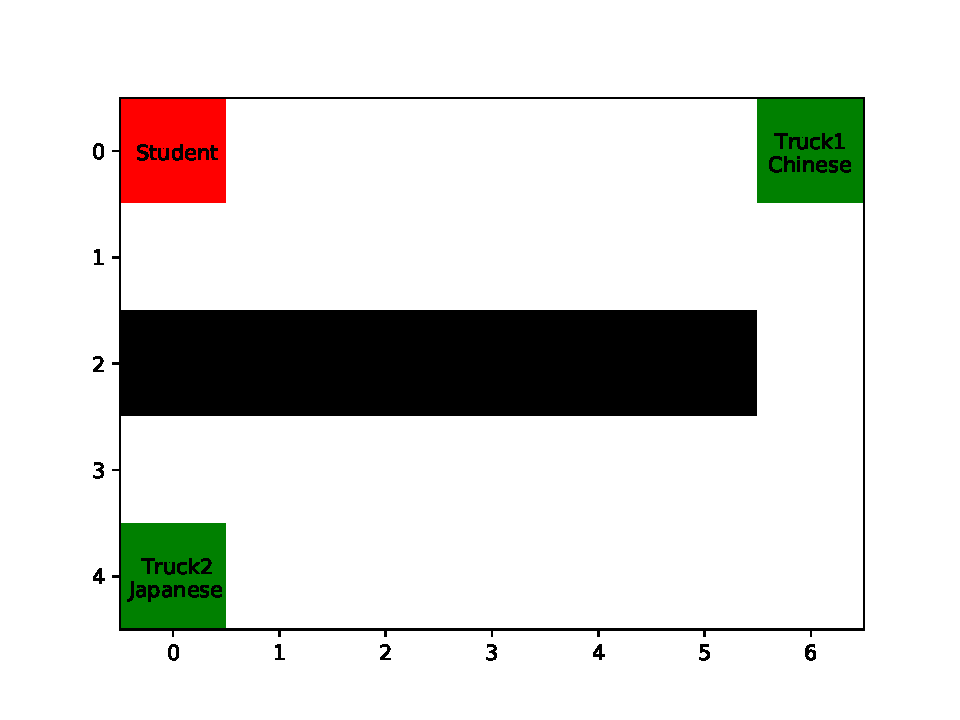
\includegraphics[scale=0.7]{./ex_env1.pdf}
    \caption{本実験における環境.図中の``Student''は学生,``Truck1''および``Truck2''は屋台を開くスペース,中央の黒色部分は壁を表す.}
    \label{fig:ex_env1}
  \end{center}
\end{figure}
7$\times$5マスで表現される環境中に壁とTruck1およびTruck2で表される屋台を開くスペースが存在し,それぞれのスペースに日本食の屋台,イタリア料理の屋台,中華料理の屋台のいずれかが出店する.環境中の学生は移動し,アシストロボットと対話をしながら食事を購入する屋台を決める状況を考える.学生は,日本食の屋台,イタリア料理の屋台,中華料理の屋台の3種類のうち2種類が出店することは知っているが,どの屋台が出店しているかは知らないため,環境中を移動しアシストロボットと対話しながら食事を買う屋台を選ぶ.学生の行動$a_t$は上,下,左,右の4方向への移動とし,発話$u_t$はアシストロボットから提示される食事に関する質問に対する学生の応答とする.信念$b_t$は,壁により観測できていない屋台に関してどの屋台が出店していると考えているか,欲求$d$は学生が3種類のそれぞれの屋台をどの程度好むかを表す.



\section{実験手順}

\par
本実験には,本研究で作成したデータセットを利用した.本データセットには,屋台の組み合わせを表す環境設定と,その環境設定で考えられる学生の行動,アシストロボットからの質問,学生の応答が含まれる.屋台の組み合わせは日本食の屋台,イタリア料理の屋台,中華料理の屋台の2つの組み合わせとする6通り,学生の行動は上,下,左,右の4方向への移動,アシストロボットからの質問は表\ref{tab:q_a}の左側に記載される4通り,学生の応答は表\ref{tab:q_a}の右側に記載される8通りである.
\begin{table}[htb]
  \begin{center}
  \caption{アシストロボットからの質問と学生の応答}
  \label{tab:q_a}
  \begin{tabular}{lll} \hline
    質問内容&\multicolumn{2}{l}{応答内容}\\\hline
    魚料理と野菜料理どちらを食べたいですか&fish&vegetable\\
    パスタと米ではどちらを食べたいですか&pasta&rice\\
    あっさりしたものと,こってりしたものどちらを食べたいですか&plain&oily\\
    辛いものと酸っぱいものではどちらを食べたいですか&spicy&sour\\\hline
  \end{tabular}
\end{center}
\end{table}
本実験では,一定時間パーティクルの尤度に大きな変化がない時およびTruck1を通り過ぎた時に質問を提示した.MIoM SCAINによって行動情報と発話情報の両方を信念と欲求の推定に活用することが有効であることを評価するために,パーティクルフィルタを用い行動情報と発話情報の一方のみを基に信念と欲求を推定するシステムUnimodal Inference of Mind SCAIN (UIoM SCAIN)を定義した.


\par
図\ref{fig:interface}に示すインターフェスを用いて,30人の実験参加者に,本データセットで指定された環境設定と行動およびアシストロボットからの質問と学生の応答を提示し,環境中の学生の信念と欲求をそれぞれ7段階で推定させた.
\begin{figure}[htbp]
  \begin{center}
    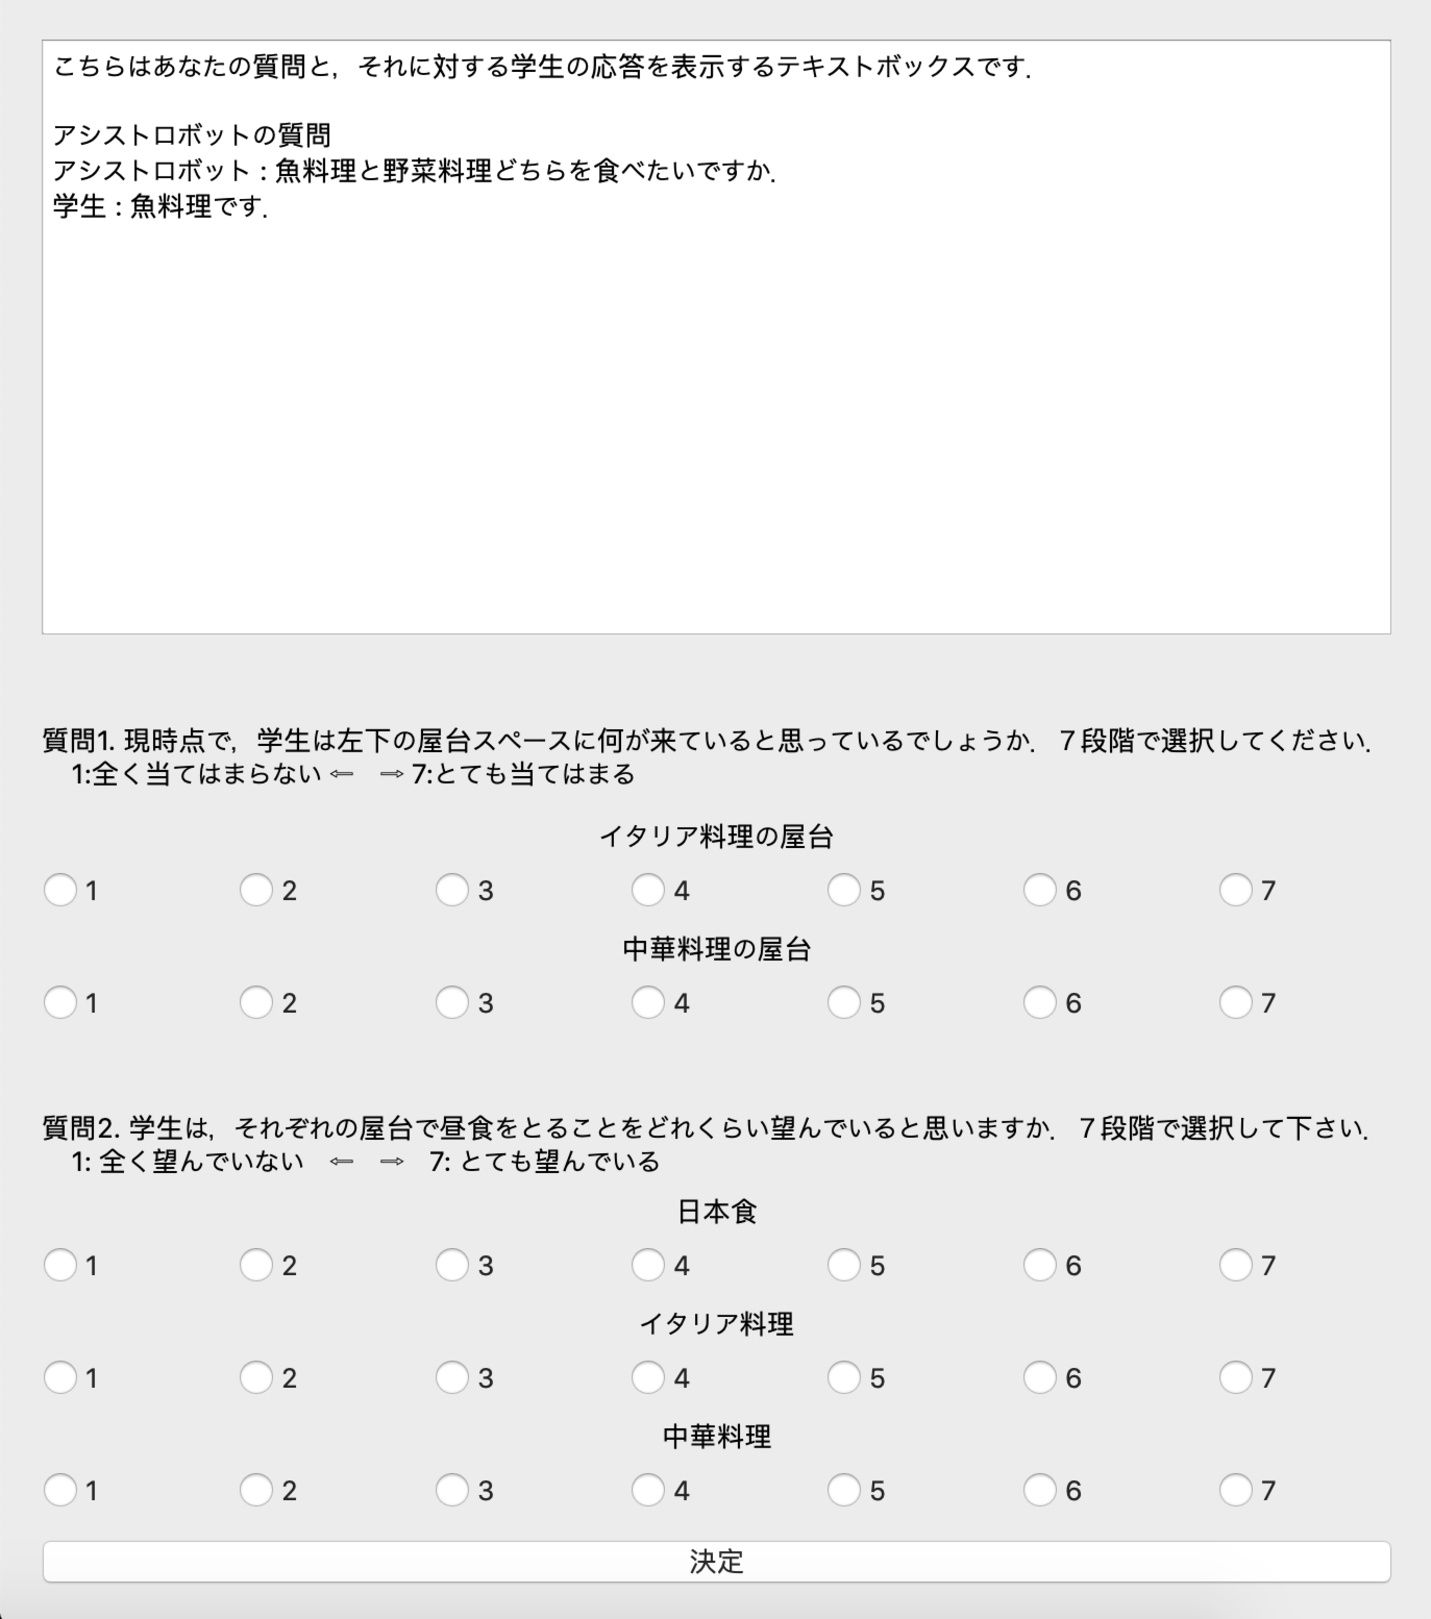
\includegraphics[scale=0.6]{./interface.pdf}
    \caption{本実験に使用したインターフェース}
    \label{fig:interface}
  \end{center}
\end{figure}
環境設定や行動の内容,アシストロボットからの質問,学生の応答に偏りがないように8つのデータを本データセットから選択し,それぞれの実験参加者に対して提示し,1つのデータに対して2回または3回推定をさせた.
また,MIoM SCAIN (action + utterance),行動情報のみを基に心的状態を推定するUIoM SCAIN (action),発話情報のみを基に心的状態を推定するUIoM SCAIN (utterance)の3つのシステムによって,環境中の学生の信念と欲求を推定し,推定結果を式(\ref{b_transform})および式(\ref{d_transform})により,7段階評価に変換した.
\begin{equation}
  \begin{split}
  \label{b_transform}
  b_t(\mathrm{Japanese})= \sum_{\substack{k\\b_t^k=\mathrm{Japanese}}} 7\cdot L^k\\
  b_t(\mathrm{Italian})=\sum_{\substack{k\\b_t^k=\mathrm{Italian}}} 7\cdot L^k\\
  b_t(\mathrm{Chinese})=\sum_{\substack{k\\b_t^k=\mathrm{Chinese}}} 7\cdot L^k\\
  \end{split}
\end{equation}

\begin{equation}
  \begin{split}
  \label{d_transform}
  d(\mathrm{Japanese})= \sum_{\substack{k\\d^k=\mathrm{Japanese}}} \frac{7}{3}\cdot L^k \cdot rank^k({\mathrm{Japanese}})\\
  d(\mathrm{Italian})= \sum_{\substack{k\\d^k=\mathrm{Italian}}} \frac{7}{3}\cdot L^k \cdot rank^k({\mathrm{Italian}})\\
  d(\mathrm{Chinese})= \sum_{\substack{k\\d^k=\mathrm{Chinese}}} \frac{7}{3}\cdot L^k \cdot rank^k({\mathrm{Chinese}})\\
  \end{split}
\end{equation}
ここで,$rank^k(\mathrm{food})$は,パーティクル$k$における欲求$d_k$を基に$\mathrm{food}$をどの程度好むかを3段階で表した値である.式(\ref{b_transform})および式(\ref{d_transform})において,尤度が最大のパーティクルのみを用いて信念や欲求を推定することをせずに,全てのパーティクルを考慮して計算を行っているのは,各パーティクルの尤度に差がない場合に対応するためである.推定を行った全タイミングで,信念推定および欲求推定のそれぞれについて,実験参加者による推定結果とMIoM SCAINおよびUIoM SCAINによる推定結果を比較し,相関係数を算出した.UIoM SCAIN (action)およびUIoM SCAIN (utterance)の尤度は,それぞれ式(\ref{uiom_a}),式(\ref{uiom_u})で計算した.それぞれのモデルについて,信念または欲求の推定において相関係数が最大になるように,式(\ref{calc_a})における$cost$の計算に用いる報酬や,式(\ref{calc_u})における関数similarity内のパラメータを設定した.
\begin{equation}
  \begin{split}
  \label{uiom_a}
  L^k({\mathrm{action}})&= \sum_{b_{t-1}^k,o_t}P(b_t^k|b_{t-1}^k,o_t)\cdot P(o_t|s_t)\cdot P(s_t|s_{t-1},a_{t-1})\\
  &\hspace{3cm}\cdot P(a_{t-1}|b_{t-1}^k,d^k)\cdot P(b_{t-1}^k,d^k,s_{t-1},a_{t-2})
  \end{split}
\end{equation}

\begin{equation}
  \begin{split}
  \label{uiom_u}
  L^k({\mathrm{utterance}})&= \sum_{b_{t-1}^k,o_t}P(b_t^k|b_{t-1}^k,o_t)\cdot P(o_t|s_t)\cdot P(s_t|s_{t-1},a_{t-1})\\
  &\hspace{3cm}\cdot P(u_{t-1}|b_{t-1}^k,d^k)\cdot P(b_{t-1}^k,d^k,s_{t-1},u_{t-2})
  \end{split}
\end{equation}


\section{実験結果}

\par
表\ref{tab:cof}に,実験参加者による信念と欲求の推定結果とUIoM SCAIN (action), UIoM SCAIN (utterance)およびMIoM SCAINによる信念と欲求の推定結果との間の相関係数を示す.
\begin{table}[htb]
  \begin{center}
  \caption{人間による推定と推定モデルの相関}
  \label{tab:cof}
  \begin{tabular}{lcc} \hline
    \multirow{2}{*}{モデル}&\multicolumn{2}{c}{相関}\\\cline{2-3}
    & \hspace{10pt} 信念 \hspace{10pt} & \hspace{10pt} 欲求 \hspace{10pt} \\ \hline
    UIoM SCAIN (action)&0.124&0.419\\
    UIoM SCAIN (utterance)&0.216&0.494\\
    MIoM SCAIN (action + utterance)&\bf0.244&\bf0.550 \\\hline
  \end{tabular}
\end{center}
\end{table}


\par
表\ref{tab:cof}より,いずれの推定システムにおいても欲求推定の相関が信念推定の相関よりも強いことがわかった.

\par
また,信念と欲求の推定の両方において,行動情報と発話情報の両方を推定に活用するMIoM SCAINが行動情報のみを推定に活用するUIoM SCAIN (action)および発話情報のみを推定に活用するUIoM SCAIN (utterance)よりも強い相関を示すことがわかった.

\par
ここで,MIoM SCAINによる信念と欲求の推定の相関とUIoM SCAINによる信念と欲求の推定の相関との間に差があると言えるかを$z$検定\cite{alma9926301497204034}によって検定した過程を示す.また,表\ref{tab:test}に検定結果を示す.

\par
まず,MIoM SCAINとUIoM SCAIN (action)の信念推定における相関に差があるかを調べる.以下のように仮説を設定する.
\begin{displaymath}
  \begin{split}
  \label{z_a_b_p}
  \mathrm{帰無仮説:MIoM\; SCAINとUIoM\; SCAIN\; (action)の信念推定の相関に差がない}\\
  \mathrm{対立仮説:MIoM\; SCAINとUIoM\; SCAIN\; (action)の信念推定の相関に差がある}\\
  \end{split}
\end{displaymath}
また,データ数を考慮して検定統計量$T$は以下のように計算される.
\begin{displaymath}
  \begin{split}
  \label{z_a_b}
  T&=\sqrt{960-3}\left(\frac{1}{2}\ln{\frac{1+0.244}{1-0.244}-\frac{1}{2}\ln{\frac{1+0.124}{1-0.124}}}\right)\\
  &=3.85\\
  \end{split}
\end{displaymath}
$\alpha=0.05$で両側検定を行う.$z\left(\frac{\alpha}{2}\right)=1.96$であり,$T=3.85>1.96$なので,帰無仮説を棄却する.よって,MIoM SCAINとUIoM SCAIN (action)の信念推定における相関に差があると言える.

\par
次に,MIoM SCAINとUIoM SCAIN (utterance)の信念推定における相関に差があるかを調べる.以下のように仮説を設定する.
\begin{displaymath}
  \begin{split}
    \label{z_a_b}
    \mathrm{帰無仮説:MIoM\; SCAINとUIoM\; SCAIN\; (utterance)の信念推定の相関に差がない}\\
    \mathrm{対立仮説:MIoM\; SCAINとUIoM\; SCAIN\; (utterance)の信念推定の相関に差がある}\\
    \end{split}
\end{displaymath}
また,データ数を考慮して検定統計量$T$は以下のように計算される.
\begin{displaymath}
  \begin{split}
  \label{z_a_b}
  T&=\sqrt{960-3}\left(\frac{1}{2}\ln{\frac{1+0.244}{1-0.244}-\frac{1}{2}\ln{\frac{1+0.216}{1-0.216}}}\right)\\
  &=0.914\\
  \end{split}
\end{displaymath}
$\alpha=0.05$で両側検定を行う.$z\left(\frac{\alpha}{2}\right)=1.96$であり,$T=0.914<1.96$なので,帰無仮説を棄却しない.よって,MIoM SCAINとUIoM SCAIN (utterance)の信念推定における相関に差があるとは言えない.

\par
次に,MIoM SCAINとUIoM SCAIN (action)の欲求推定における相関に差があるかを調べる.以下のように仮説を設定する.
\begin{displaymath}
  \begin{split}
  \label{z_a_b}
  \mathrm{帰無仮説:MIoM\; SCAINとUIoM\; SCAIN\; (action)の欲求推定の相関に差がない}\\
  \mathrm{対立仮説:MIoM\; SCAINとUIoM\; SCAIN\; (action)の欲求推定の相関に差がある}\\
  \end{split}
\end{displaymath}
また,データ数を考慮して検定統計量$T$は以下のように計算される.
\begin{displaymath}
  \begin{split}
  \label{z_a_b}
  T&=\sqrt{1800-3}\left(\frac{1}{2}\ln{\frac{1+0.549}{1-0.549}-\frac{1}{2}\ln{\frac{1+0.419}{1-0.419}}}\right)\\
  &=7.23\\
  \end{split}
\end{displaymath}
$\alpha=0.05$で両側検定を行う.$z\left(\frac{\alpha}{2}\right)=1.96$であり,$T=7.23>1.96$なので,帰無仮説を棄却する.よって,MIoM SCAINとUIoM SCAIN (action)の欲求推定における相関に差があると言える.

\par
最後に,MIoM SCAINとUIoM SCAIN (utterance)の欲求推定における相関に差があるかを調べる.以下のように仮説を設定する.
\begin{displaymath}
  \begin{split}
  \label{z_a_b}
  \mathrm{帰無仮説:MIoM\; SCAINとUIoM\; SCAIN\; (utterance)の欲求推定の相関に差がない}\\
  \mathrm{対立仮説:MIoM\; SCAINとUIoM\; SCAIN\; (utterance)の欲求推定の相関に差がある}\\
  \end{split}
\end{displaymath}
また,データ数を考慮して検定統計量$T$は以下のように計算される.
\begin{displaymath}
  \begin{split}
  \label{z_a_b}
  T&=\sqrt{1800-3}\left(\frac{1}{2}\ln{\frac{1+0.549}{1-0.549}-\frac{1}{2}\ln{\frac{1+0.494}{1-0.494}}}\right)\\
  &=3.20\\
  \end{split}
\end{displaymath}
$\alpha=0.05$で両側検定を行う.$z\left(\frac{\alpha}{2}\right)=1.96$であり,$T=3.20>1.96$なので,帰無仮説を棄却する.よって,MIoM SCAINとUIoM SCAIN (utterance)の欲求推定における相関に差があると言える.

\begin{table}[htb]
  \begin{center}
  \caption{信念および欲求の推定におけるMIoM SCAINとUIoM SCAINの有意差検定}
  \label{tab:test}
  \begin{tabular}{lcc} \hline
    &信念&欲求\\\cline{2-3}
    & \hspace{10pt} MIoM SCAIN \hspace{10pt} & \hspace{10pt} MIoM SCAIN \hspace{10pt} \\ \hline
    UIoM SCAIN (action)&差があると言える&差があると言える\\
    UIoM SCAIN (utterance)&差があると言えない&差があると言える\\\hline
  \end{tabular}
\end{center}
\end{table}

\chapter{結論}
本論文では,MIoM SCAINによりマルチモーダルな心的状態推定について検討した.実験の結果,行動情報と発話情報の両方を心的状態の推定に用いることが有効であることを示した.今後の展望としては,より実世界に近い環境設定や三次元の行動および多種多様な発話を扱えるようにMIoM SCAINを拡張したいと考えている.

%%
%%

%
% 謝辞
%
\chapter*{謝辞}
\addcontentsline{toc}{chapter}{謝辞}
\baselineskip = 20pt

\begin{verbatimtab}
	本研究を進めるにあたり、研究の機会及び貴重なご意見を頂きました、
			慶應義塾大学理工学部 今井 倫太 教授
に深く感謝致します。


	論文の査読をして頂き、細部にわたって御意見を頂きました
			理工学研究科博士課程2年 福地 庸介 氏
			理工学部研究員 前川知行 氏
に厚く御礼申し上げます。

  
	実験に御協力頂いた被験者の方々に心より御礼申し上げます。



最後に日頃から御指導、御協力下さいました今井研究室の皆様に心より感謝いたします。


							令和3年1月
\end{verbatimtab}

% \begin{verbatimtab}
% 	本研究を進めるにあたり、研究の機会及び貴重なご意見を頂きました、
% 			慶應義塾大学理工学部 今井 倫太 准教授
% 			慶應義塾大学理工学部 大澤 博隆 助教
% に深く感謝致します。


% 	論文の査読をして頂き、細部にわたって御意見を頂きました
% 			理工学部研究科修士課程1年 尾形 正泰 氏
% に厚く御礼申し上げます。

%   
% 	実験に御協力頂いた被験者の方々に心より御礼申し上げます。



% 最後に日頃から御指導、御協力下さいました今井研究室の皆様に心より感謝いたします。


% 							平成24年1月
% \end{verbatimtab}
    %謝辞

\bibliography{reference}     %参考文献

\end{document}
